\chapter{Week4}
\section{Monday for MAT3040}\index{Monday_lecture}

\subsection{Quotient Spaces}

Now we aim to divide a big \emph{vector space} into many pieces of slices. 
\begin{itemize}
\item
For example, the Cartesian plane can be expressed as union of set of vertical lines as follows:
\[
\mathbb{R}^2 = \bigcup_{m\in\mathbb{R}}\left\{\begin{pmatrix}
m\\0
\end{pmatrix}+
\Span\{(0,1)\}\}
\right\}
\]
\item
Another example is that the set of integers can be expressed as union of three sets:
\[
\mathbb{Z}
=
Z_1\cup Z_2\cup Z_3,
\]
where $Z_i$ is the set of integers $z$ such that $z\text{ mod }3 = i$.
\end{itemize}

\begin{definition}[Coset]
Let $V$ be a vector space and $W\le V$. For any element $\bm v\in V$, the \emph{(right) coset} determined by $\bm v$ is the set
\[
\bm v+W:=\{\bm v+\bm w\mid\bm w\in W\}
\]
\end{definition}

For example, consider $V=\mathbb{R}^3$ and $W=\Span\{(1,2,0)\}$. Then the coset determined by $\bm v=(5,6,-3)$ can be written as
\[
\bm v+W=\left\{(5+t,6+2t,-3)\mid t\in\mathbb{R}\right\}
\]
It's interesting that the coset determined by $\bm v'=\{(4,4,-3)\}$ is exactly the same as the coset shown above:
\[
\bm v'+W=\left\{(4+t,4+2t,-3)\mid t\in\mathbb{R}\right\}=\bm v+W.
\]

Therefore, write the exact expression of $\bm v+W$ may sometimes become tedious and hard to check the equivalence. We say $\bm v$ is a \emph{representative} of a coset $\bm v+W$.

\begin{proposition}\label{pro:4:1}
Two cosets are the same iff the subtraction for the corresponding representatives is in $W$, i.e., 
\[
\bm v_1+W=\bm v_2+W
\Longleftrightarrow
\bm v_1-\bm v_2\in W
\]
\end{proposition}
\begin{proof}
\textit{Necessity.}
Suppose that $\bm v_1+W=\bm v_2+W$, then $\bm v_1+\bm w_1=\bm v_2+\bm w_2$ for some $\bm w_1,\bm w_2\in W$, which implies
\[
\bm v_1-\bm v_2=\bm w_2-\bm w_1\in W
\]
\textit{Sufficiency.}
Suppose that $\bm v_1-\bm v_2=\bm w\in W$. It suffices to show $\bm v_1+W\subseteq\bm v_2+W$.
For any $\bm v_1+\bm w'\in \bm v_1+W$, this element can be expressed as
\[
\bm v_1+\bm w'=(\bm v_2+\bm w)+\bm w'=\bm v_2+\underbrace{(\bm w+\bm w')}_{\text{belong to $W$}}\in \bm v_2+W.
\]
Therefore, $\bm v_1+W\subseteq \bm v_2+W$. Similarly we can show that $\bm v_2+W\subseteq \bm v_1+W$.
\end{proof}
\textit{Exercise: }Two cosets with representatives $\bm v_1,\bm v_2$ have no intersection iff $\bm v_1-\bm v_2\notin W$.

\begin{definition}[Quotient Space]
The \emph{quotient space} of $V$ by the subspace $W$, is the collection of all cosets $\bm v+W$, denoted by $V/ W$.
\end{definition}
To make the quotient space a vector space structure, we define the addition and scalar multiplication on $V/ W$ by:
\begin{align*}
(\bm v_1+W)+(\bm v_2+W)&:=(\bm v_1+\bm v_2)+W\\
\alpha\cdot (\bm v+W)&:=(\alpha\cdot\bm v) + W
\end{align*}

For example, consider $V=\mathbb{R}^2$ and $W=\Span\{(0,1)\}$. Then note that
\begin{align*}
\left(
\begin{pmatrix}
1\\0
\end{pmatrix}+W
\right)
+
\left(
\begin{pmatrix}
2\\0
\end{pmatrix}+W
\right)
&=
\left(
\begin{pmatrix}
3\\0
\end{pmatrix}+W
\right)\\
\pi\cdot\left(
\begin{pmatrix}
1\\0
\end{pmatrix}+W
\right)
&=
\left(
\begin{pmatrix}
\pi\\0
\end{pmatrix}+W
\right)
\end{align*}

\begin{proposition}
The addition and scalar multiplication is well-defined.
\end{proposition}
\begin{proof}
\begin{enumerate}
\item
Suppose that
\begin{equation}\label{Eq:4:1}
\left\{
\begin{aligned}
\bm v_1+W&=\bm v_1'+W\\
\bm v_2+W&=\bm v_2'+W
\end{aligned}
\right.,
\end{equation}
and we need to show that $(\bm v_1+\bm v_2)+W=(\bm v_1'+\bm v_2')+W$. 

From (\ref{Eq:4:1}) and proposition~(\ref{pro:4:1}), we imply
\[
\bm v_1-\bm v_1'\in W,\quad
\bm v_2-\bm v_2'\in W
\]
which implies
\[
(\bm v_1-\bm v_1')+(\bm v_2-\bm v_2')=(\bm v_1+\bm v_2) - (\bm v_1'+\bm v_2')\in W
\]

By proposition~(\ref{pro:4:1}) again we imply $(\bm v_1+\bm v_2)+W=(\bm v_1'+\bm v_2')+W$
\item
For scalar multiplication, similarly, we can show that $\bm v_1+W=\bm v_1'+W$ implies $\alpha\bm v_1+W=\alpha\bm v_1'+W$ for all $\alpha\in\mathbb{F}$.

\end{enumerate}

\end{proof}

\begin{proposition}
The canonical projection mapping
\[
\begin{aligned}
\pi_W:&V\to V/ W,\\
&\bm v\mapsto\bm v+W,
\end{aligned}
\]
is a \emph{surjective} \emph{linear transformation} with $\ker(\pi_W) = W$.
\end{proposition}
\begin{proof}
\begin{enumerate}
\item
First we show that $\ker(\pi_W)=W$:
\[
\pi_W(\bm v)=0\implies
\bm v+W=\bm0_{V/ W}\implies
\bm v+W=\bm0+W\implies \bm v=(\bm v-\bm0)\in W
\]
Here note that the zero element in the quotient space $V/ W$ is the coset with representative $\bm0$.
\item
For any $\bm v_0+W\in V/ W$, we can construct $\bm v_0\in V$ such that $\pi_W(\bm v_0)=\bm v_0+W$. Therefore the mapping $\pi_W$ is surjective.
\item
To show the mapping $\pi_W$ is a linear transformation, note that
\begin{align*}
\pi_W(\alpha\bm v_1+\beta\bm v_2)&=(\alpha\bm v_1+\beta\bm v_2)+W\\
&=(\alpha\bm v_1+W)+(\beta\bm v_2+W)\\
&=\alpha(\bm v_1+W)+\beta(\bm v_2+W)\\
&=\alpha\pi_W(\bm v_1)+\beta\pi_W(\bm v_2)
\end{align*}

\end{enumerate}


\end{proof}



\subsection{First Isomorphism Theorem}
The key of linear algebra is to solve the linear system $\bm A\bm x=\bm b$ with $\bm A\in\mathbb{R}^{m\times n}$. 
The general step for solving this linear system is as follows:
\begin{enumerate}
\item
Find the solution set for $\bm A\bm x=\bm0$, i.e., the set $\ker(\bm A)$
\item
Find a particular solution $\bm x_0$ such that $\bm A\bm x_0=\bm b$.
\end{enumerate}
Then the general solution set to this linear system is $\bm x_0+\ker(\bm A)$, which is a coset in the space $\mathbb{R}^n/ \ker(\bm A)$. Therefore, to solve the linear system $\bm{Ax}=\bm b$ suffices to study the quotient space $\mathbb{R}^n/ \ker(\bm A)$:

\begin{proposition}[Universal Property I]
Suppose that $T:V\to W$ is a linear transformation, and that $V'\le\ker(T)$. Then the mapping
\begin{align*}
\tilde{T}&:V/ V'\to W\\
&\bm v+V'\mapsto T(\bm v)
\end{align*}
is a well-defined linear transformation. As a result, the diagram below commutes:
\begin{figure}[H]
\centering
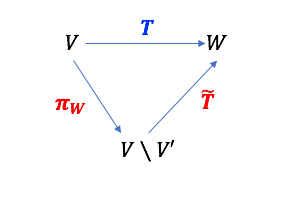
\includegraphics[width=0.5\textwidth]{week4/p_1}
\end{figure}
In other words, we have $T = \tilde{T}\circ \pi_W$.
\end{proposition}

\begin{proof}
First we show the well-definedness. Suppose that $\bm v_1+V'=\bm v_2+V'$ and suffices to show $\tilde T(\bm v_1+V')=\tilde T(\bm v_2+V')$, i.e., $T(\bm v_1)=T(\bm v_2)$. By proposition~(\ref{pro:4:1}), we imply
\[
\bm v_1-\bm v_2\in V'\le\ker(T)\implies
T(\bm v_1-\bm v_2)=\bm0\implies T(\bm v_1)-T(\bm v_2)=\bm0.
\]
Then we show $\tilde(T)$ is a linear transformation:
\begin{align*}
\tilde{T}(\alpha(\bm v_1+V')  + \beta(\bm v_2+V'))&=\tilde{T}((\alpha\bm v_1+\beta\bm v_2)+V')\\
&=T(\alpha\bm v_1+\beta\bm v_2)\\
&=\alpha T(\bm v_1)+\beta T(\bm v_2)\\
&=\alpha\tilde{T}(\bm v_1+V')+\beta\tilde{T}(\bm v_2+V')
\end{align*}
\end{proof}

Actually, if we let $V'=\ker(T)$, the mapping $\tilde{T}:V/ V'\to T(V)$ forms an isomorphism, In particular, if further $T$ is surjective, then $T(V)=W$, i.e., the mapping $\tilde{T}:V/ V'\to W$ forms an isomorphism.
\begin{theorem}[First Isomorphism Theorem]
Let $T:V\to W$ be a surjective linear transformation. Then the mapping 
\begin{align*}
\tilde{T}&:V/ \ker(T)\to W\\
&\bm v+\ker(T)\mapsto T(\bm v)
\end{align*}
is an isomorphism.
\end{theorem}
\begin{proof}
\textit{Injectivity.} Suppose that $\tilde{T}(\bm v_1+\ker(T)) = \tilde{T}(\bm v_2+\ker(T))$, then we imply
\[
T(\bm v_1)=T(\bm v_2)\implies T(\bm v_1-\bm v_2)=\bm0_W\implies\bm v_1-\bm v_2\in\ker(T),
\]
i.e., $\bm v_1+\ker(T)=\bm v_2+\ker(T)$.

\textit{Surjectivity.} For $\bm w\in W$, due to the surjectivity of $T$, we can find a $\bm v_0$ such that $T(\bm v_0)=\bm w$. Therefore, we can construct a set $\bm v_0+\ker(T)$ such that
\[
\tilde{T}(\bm v_0+\ker(T))=\bm w.
\]
\end{proof}


















